\section{Siciliano, Khatib - Handbook of Robotics, ch. 7, Force Control - 2008}
\subsection*{Impedance Control}
\subsection*{Admittance Control}
\subsubsection*{Difference between impedance and admittance control}

\begin{itemize}
\item \textit{impedance control}: when, given a certain displacement, a corresponding reaction force is imposed. The impedance controller feedback is an acceleration in the task space that, with inverse dynamics, can be translated into a force in the joint space (figure \ref{ImpContr}).
\item \textit{admittance control}: as opposite to impedance control here, given a certain interaction force, a corresponding motion (position and velocity) is imposed (figure \ref{admitContr}). This can be done be decoupling the impedance controller into two parts, one in charge of tracking the reference motion and on in charge of a compliant frame. This compliant frame coincides with the desired frame when there is no interaction. In presence of interaction instead the motion controller will rigidly track the reference given by the compliant frame.
\item \textit{damping control}
\item \textit{stiffness control}
\end{itemize}

\begin{figure}[h]
  \centering
  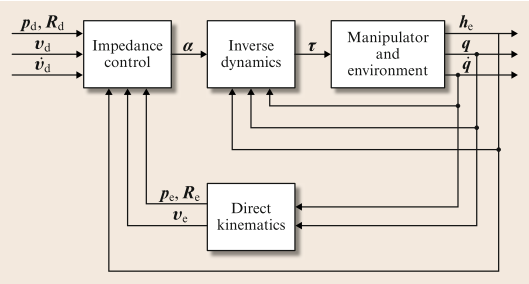
\includegraphics[width=100mm]{ImpedanceControl}
  \caption{Impedance control}
  \label{ImpContr}
\end{figure}
\begin{figure}[h]
  \centering
  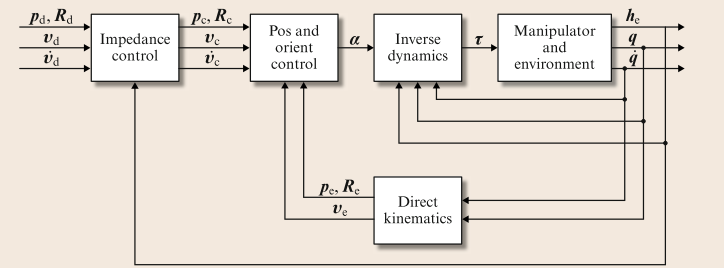
\includegraphics[width=100mm]{AdmittanceControl}
  \caption{Admittance control}
  \label{admitContr}
\end{figure}